\documentclass[tikz,border=3pt]{standalone}
\usepackage[utf8]{inputenc}
\usepackage[T1]{fontenc}
\usepackage{lmodern}
\renewcommand{\familydefault}{\sfdefault}
\usepackage{sansmath}\sansmath
\usepackage{chemfig}
\usepackage{pgfplots}\pgfplotsset{compat=1.18,/pgf/number format/use comma,/pgf/number format/1000 sep={.}}
\usetikzlibrary{arrows.meta,calc,positioning,decorations.pathmorphing,patterns}
% paleta del sitio
\definecolor{nar}{HTML}{E8680C}\definecolor{narc}{HTML}{FFB35C}\definecolor{hielo}{HTML}{FFF3E8}
\definecolor{tinta}{HTML}{1D1D1F}\definecolor{gris}{HTML}{6E6E73}\definecolor{lila}{HTML}{7C5CF0}
\definecolor{azul}{HTML}{2F6FD6}\definecolor{menta}{HTML}{17A673}\definecolor{coral}{HTML}{E8342A}
\begin{document}
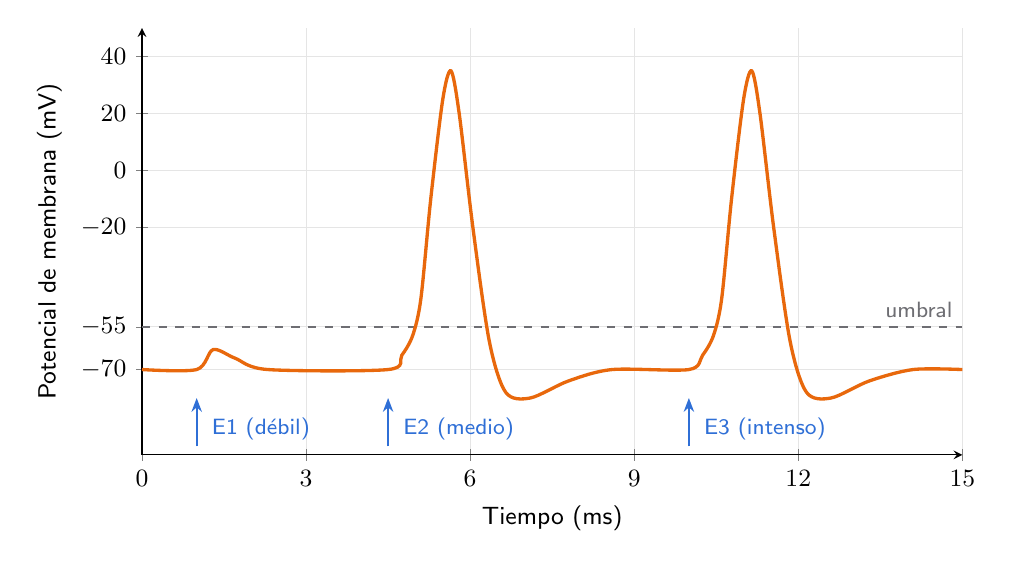
\begin{tikzpicture}[font=\small]
\begin{axis}[axis lines=left,grid=major,grid style={gray!20},xlabel={Tiempo (ms)},ylabel={Potencial de membrana (mV)},
  width=12cm,height=7cm,xmin=0,xmax=15,ymin=-100,ymax=50,ytick={-70,-55,-20,0,20,40},xtick={0,3,...,15},clip=false]
\addplot[gris,dashed,thick,domain=0:15] {-55};
\addplot[nar,very thick,smooth,tension=0.5] coordinates {(0,-70)(1,-70)(1.3,-63)(1.7,-66)(2.3,-70)(4.5,-70)(4.75,-65)(4.95,-58)(5.1,-45)(5.28,-10)(5.5,25)(5.65,35)(5.8,20)(6.05,-20)(6.35,-60)(6.65,-78)(7.1,-80)(7.8,-74)(8.6,-70)(10,-70)(10.25,-65)(10.45,-58)(10.6,-45)(10.78,-10)(11.0,25)(11.15,35)(11.3,20)(11.55,-20)(11.85,-60)(12.15,-78)(12.6,-80)(13.3,-74)(14.1,-70)(15,-70)};
\node[anchor=south east,text=gris,font=\footnotesize] at (axis cs:15,-55) {umbral};
\draw[-{Stealth[length=5pt]},azul,thick] (axis cs:1,-97) -- (axis cs:1,-80);
\draw[-{Stealth[length=5pt]},azul,thick] (axis cs:4.5,-97) -- (axis cs:4.5,-80);
\draw[-{Stealth[length=5pt]},azul,thick] (axis cs:10,-97) -- (axis cs:10,-80);
\node[anchor=west,text=azul,font=\footnotesize] at (axis cs:1.1,-91) {E1 (débil)};
\node[anchor=west,text=azul,font=\footnotesize] at (axis cs:4.6,-91) {E2 (medio)};
\node[anchor=west,text=azul,font=\footnotesize] at (axis cs:10.1,-91) {E3 (intenso)};
\end{axis}
\end{tikzpicture}
\end{document}
